% Slides for 2025-07-22
% To create a slide, use the following:
% \begin{frame}{TITLE}
%     BODY
% \end{frame}

% To create a slide with a bullet list, use the following:
% \begin{frame}{TITLE}
%     \begin{itemize}
%         \item ITEM 1
%         \item ITEM 2
%     \end{itemize}    
% \end{frame}

% To create a slide with numbered list, use the following:
% \begin{frame}{TITLE}
%     \begin{enumerate}
%         \item ITEM 1
%         \item ITEM 2
%     \end{enumerate}
% \end{frame}

% To create a slide with a graphic:
% 1. Add the graphic to this folder (named picture.png)
% 2. Use the following:
% \begin{frame}{TITLE}
%     \centering
%     \includegraphics[height=0.7\textheight,width=0.7\textwidth,keepaspectratio]{picture.png}
% \end{frame}

% To create a slide with two columns, use the following:
% \begin{frame}{TITLE}
%     \begin{columns}
%         \begin{column}{0.5\textwidth}
%             COLUMN 1 BODY
%         \end{column}
%         \begin{column}{0.5\textwidth}
%             COLUMN 2 BODY
%         \end{column}
%     \end{columns}
% \end{frame}
\begin{frame}{Meeting with the Aburto Lab}
    \begin{columns}
        \begin{column}{0.5\textwidth}
            \textbf{\uline{Their System}}\\
            
\includegraphics[width=0.5\textwidth]{images/esri.png}
            \begin{itemize}
                \item Built-in models as a part of ArcGIS
                \item 2m resolution
                \item Labeling a single large image
            \end{itemize}
        \end{column}
        \begin{column}{0.5\textwidth}
            \textbf{\uline{How can we help?}}\\
            \begin{itemize}
                \item Segmentation of drone imagery
                \item Supersampling would also help with handling satellite imagery
                \item Another task: labeling hazards (roads, buildings, etc.)
            \end{itemize}
        \end{column}
    \end{columns}
\end{frame}

\begin{frame}{Next Steps for Aburto Lab}
    \begin{itemize}
        \item Get access to their additional drone
        \item Potentially compare our model to the ArcGIS model
        \item Adapt our model for 2m resolution upscaling
    \end{itemize}

    
\end{frame}

\begin{frame}{Diffusion Layer Training}
  \begin{itemize}
      \item x0: clean latent space. x1: noisy latent space. xt: intermediate latent space
      \item training: predict noise vector x0 to xt
      \item evaluation: iteratively backtrack from x1 to x0 to get \texttt{x0\_pred}
      \item benchmarking: loss from \texttt{x0\_pred} and x0 should decrease through denoising process
  \end{itemize}    
\end{frame}

\begin{frame}{Metrics}
  \centering
  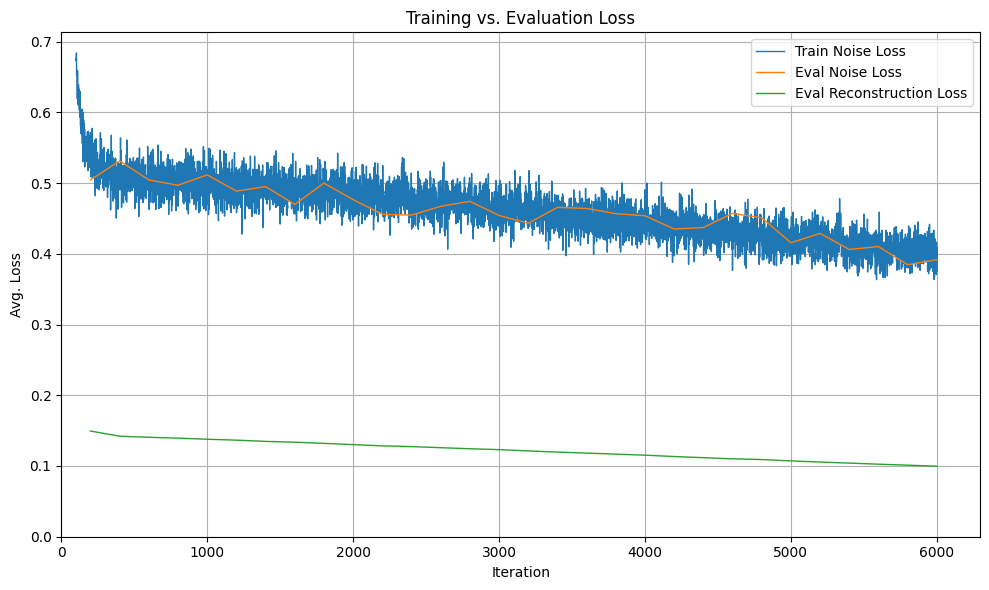
\includegraphics[height=0.7\textheight,width=0.7\textwidth,keepaspectratio]{images/diff4_loss.png}
\end{frame}

\begin{frame}{Metrics}
  \centering
  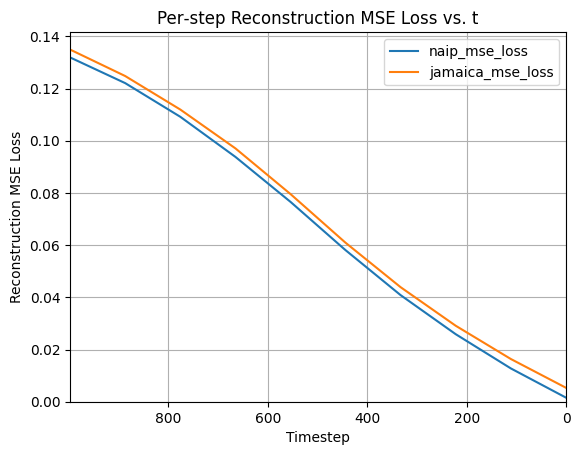
\includegraphics[height=0.7\textheight,width=0.7\textwidth,keepaspectratio]{images/diff4_reconstruct.png}
\end{frame}
